%!TEX root = ../main.tex

\chapter{Schematic Editor}

The first step in every project is schematic capture.
If this term is unfamiliar, we are referring to the process of laying out the components and connections between them in logical, well-defined fashion.
You may have only the barest idea of the circuit aspects or you may have the major aspects already sketched on paper;
whatever your situation, transferring the schematic into KiCad begins with the Schematic Editor.

Before we dive into the simplistic aspects of the schematic editor, it will pay us dividends later to properly understand how the schematic editor views more complex schematics.
This will allow you to structure the schematic in your mind more closely to how Schematic Editor expects.

\section{Hierarchical Schematics Explained}

The basic, underlying paradigm of the Schematic Editor is the idea of \textit{hierarchical schematics}.
If the overall schematic represents the full circuit that will exist on the circuit board at the end of production, then the hierarchy provides a logical grouping of similar component sets.
This allows you to reuse common subsets throughout your design.
The hierarchy also explicitly structures your schematics as a top-down tree.
\begin{figure}
	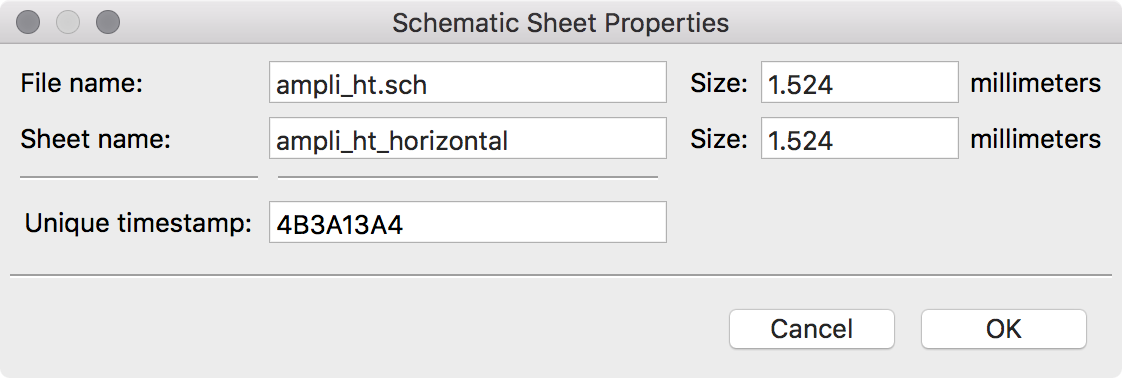
\includegraphics{chapter5/subsheet.png}
	\caption[Sub-Sheets]{The subsheet dialog specifies the file name, sheet name and a unique timestamp.}
\end{figure}

At the root of the tree, is the first schematic sheet you open, usually with the same name as your project and the extension `\textbf{.sch}'.
Off of this root, you can create \textit{sub-sheets} that are placed in the root sheet.
The sub-sheet has both a ``File name'' and a ``Sheet name''.
The File name is the name of the sub-sheet on the underlying filesystem.
This is the name you will see if you open your project folder outside of KiCad.
The Sheet name is the internal reference of the specific \textit{instance} of the sub-sheet in KiCad.

One of the primary benefits of this setup is the ability to organize the relationship between subsheets.
Instead of utilizing global net labels to connect disparate elements between sheets, you can use hierarchical subsheets layout the explicit connection between schematic elements.

It can also allow you to create and re-use common elements through and between projects.
This will be useful when we begin discussing design reuse in section \ref{sec:reuse}.



\section{Understanding the Schematic Editor}

When you first open the schematic editor, you are presented with a blizzard of information.
In KiCad, the majority of functions are accessed using buttons and hotkeys.
Unlike many programs, where functionality is often buried in sub-menus, KiCad prefers to expose its controls up front.
This has the benefit of providing easy access to virtually all commands, and the drawback of an overwhelming first impression.

\begin{figure*}
    \begin{tikzpicture}[baseline]
    \begin{scope}
        \node[anchor=south west,inner sep=0] (image) at (0,0) 
        	{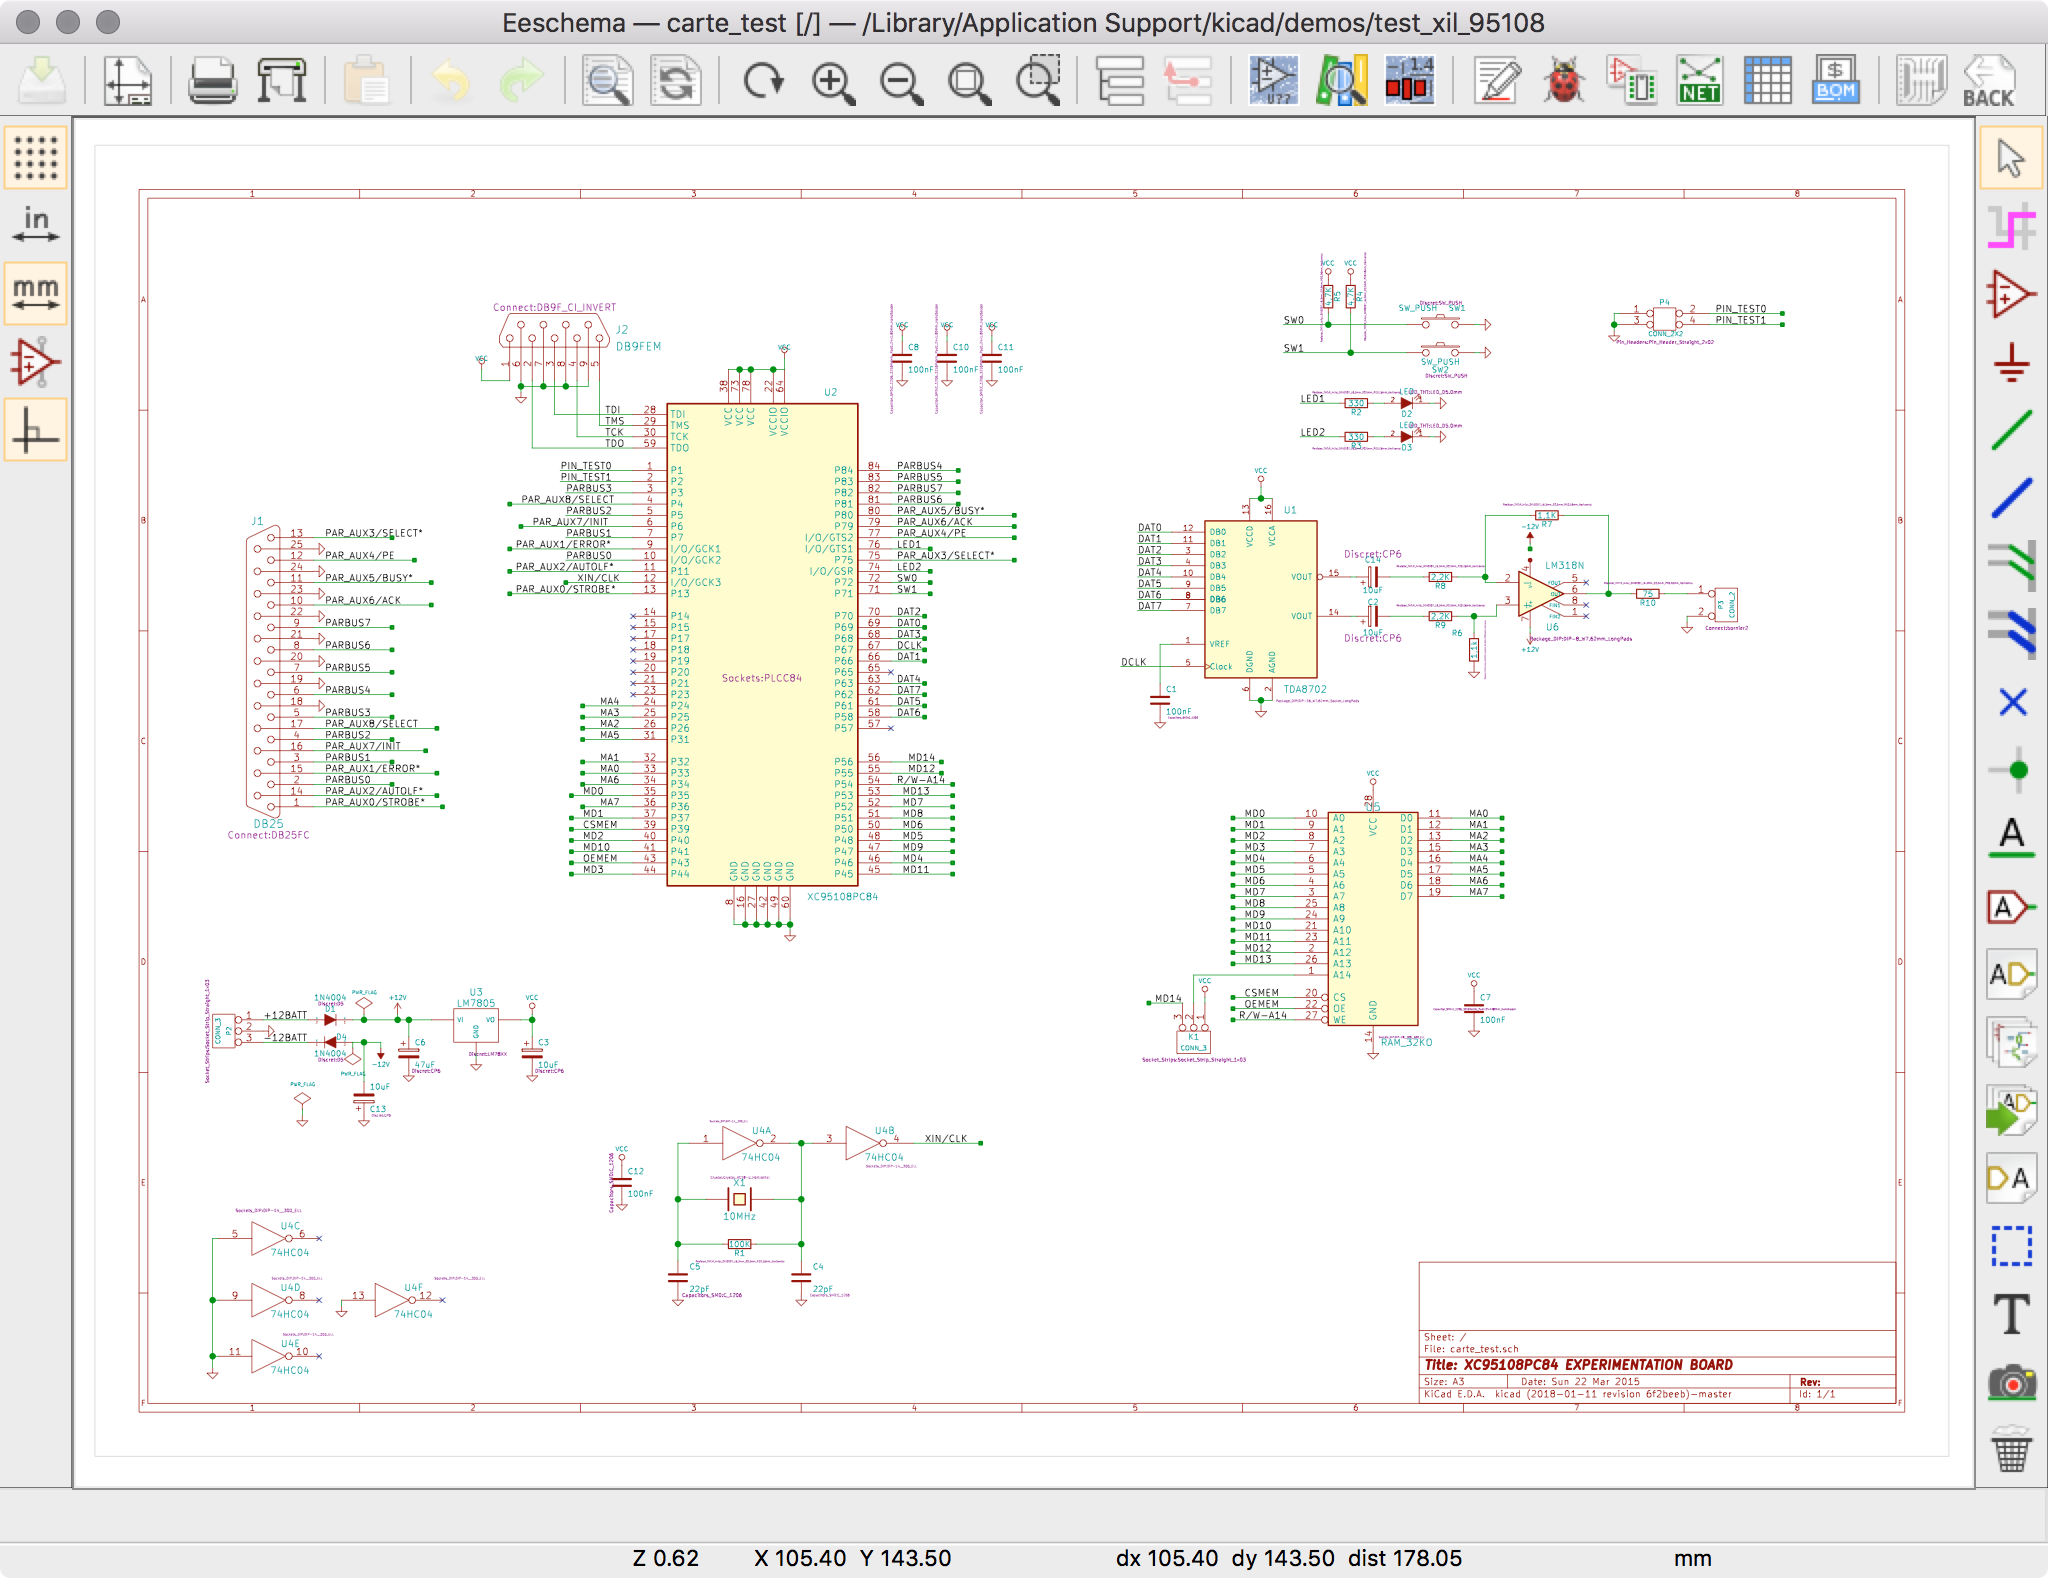
\includegraphics[width=4.5in]{chapter5/eeschema-main.png}};
        \begin{scope}[x={(image.south east)},y={(image.north west)}]
            \node [anchor=south] (file) at (0.08,1.0) {\large File\strut };
            \node [anchor=south] (edit) at (0.2575,1.0) {\large Edit\strut };
            \node [anchor=south] (view) at (0.438,1.0) {\large View\strut };
            \node [anchor=south] (app) at (0.763,1.0) {\large Applications\strut };
            \node [anchor=south, rotate=-90] (tools) at (1.0,0.5) {\large Schematic Tools};
            \node [anchor=north, rotate=-90] (options) at (0.0,0.5) {\large Display Options};
            \node [above left=-2pt] (coord) at (0.0,0.0) {\large Coordinates };
            
%            \draw[help lines,xstep=.05,ystep=.05] (0,0) grid (1,1);
            \draw[red,thick,rounded corners] (0.0,0.923) rectangle (0.155,0.97);
            \draw[red,thick,rounded corners] (0.162,0.923) rectangle (0.35,0.97);
            \draw[red,thick,rounded corners] (0.357,0.923) rectangle (0.525,0.97);
            \draw[red,thick,rounded corners] (0.60,0.923) rectangle (1.0,0.97);
            \draw[black!80,thick, dashed, rounded corners] (0.961,0.92) rectangle (1.0,0.05);
            \draw[black!80,thick, dashed, rounded corners] (0.0,0.92) rectangle (0.039,0.7);
            \draw [-latex, thick, red] ([yshift=-2pt]file.base) -- ++(0,-0.05);
            \draw [-latex, thick, red] ([yshift=-2pt]view.base) -- ++(0,-0.05);
            \draw [-latex, thick, red] ([yshift=-2pt]edit.base) -- ++(0,-0.05);
            \draw [-latex, thick, red] ([yshift=-2pt]app.base) -- ++(0,-0.05);
            \draw [-latex, thick, dashed, black!80] (tools.west) to[out=90, in=-20] (1.0,0.85);
            \draw [-latex, thick, dashed, black!80] (options.west) to[out=90, in=-160] (0.0,0.85);
            \draw [-latex, thick, dotted, black!80] (coord.east) -- ++(0.15,0.0);
        \end{scope}
    \end{scope}
    \end{tikzpicture}
	
	\caption[fig:eeschema]{The Eeschema main window.  Control and execution buttons are on the top, options buttons are in the left vertical bar and tools buttons are in the right vertical bar. }
\end{figure*}

Looking at the Eeschema window in Figure \ref{fig:eeschema}, you can see this division.
The ``Display Options'' toolbar on the left consists of buttons and are either enabled or disabled, depending on your working preferences.

\newpage
\iconstart{grid.svg}\textsc{Show Grid} icon controls whether the grid dots are shown on the schematic or not.
Note that this does not change whether your elements snap to the grid; this is always enabled for Eeschema.

\iconstarts{unit_inch.svg}{unit_mm.svg}\textsc{Unit Selection} icons allow you to choose either imperial (inch and mil) or metric (millimeter) units for the dimensions.  
When selecting one of these icons, you don't change the grid size, just the representation.
Note that while you can change the representation of the grid size, you cannot change the base unit.
That is to say, the grid is always in units of mil (thousandth of an inch) and their multiples.
This is an historical artifact of the underlying schematic format.
\sidenote[][-10ex]{Originally, Eeschema and Pcbnew used similar file formats.  
When they were designed in the early 1990s, the vast majority of components were only available in imperial pitch.
Therefore it made sense to have the base unit be the mil.
This limitation no longer exists for pcbnew and there are plans in the works to change it for Eeschema in version 6.}

\iconstart{cursor_shape.svg}\textsc{Show Cross-hairs} button changes how the cursor is displayed on the canvas.
Enabling this button will change the cursor shape to a cross-hair whose whiskers extend across the canvas.
\sidenote{This option is not available on the MacOS version.}
You may want to enable this option when you are editing a large schematic and would like to ensure you are placing the corner of a line at the same horizontal or vertical position as the position where you want to connect it.

\iconstart{hidden_pin.svg}\textsc{Hidden Pins} button shows pins that are marked ``hidden'' in light grey on the schematic.
Hidden pins can be useful for multiple pins that share a function and for pins that are not meant to be connected\sidenote{\url{http://kicad-pcb.org/libraries/klc/S4.6/}}.
Historically, hidden pins were also used for common connection pins such as \textbf{VCC} or \textbf{GND}.
This caused many issues as Eeschema connects hidden pins to wires that cross them, so users would sometimes find their netlist cross-linked by a wire that inadvertently crossed a hidden pin.
While new library symbols in the official distribution have explicitly separated the hidden connection pins per KLC4.6, there exist some historical symbols, notably in the \texttt{Logic\_TTL\_IEEE} and \texttt{Logic\_74xgxx} libraries that have not be updated to the new standard.
Selecting this view option is a good way to verify you haven't been caught by this particular issue

\iconstart{lines90.svg}\textsc{Restrict Angles} button will keep your Eeschema wires either horizontal or vertical.
In Eeschema, all lines both start and end on grid points.
When lines are not restricted to the two axes, it is difficult to connect a second line to the middle.
Restricting the direction of new lines keeps your circuit clean and connectable.
There are always times when you might want off-axis wires.
Most times, however, keeping this enabled enforces good habits.

\subsection{Eeschema Tools Icons}
Next, let's look at the tools available in Eeschema.
These are accessible using the toolbar on the right of your schematic screen.
They are also accessible using the \menu{Place} menu.

\iconstart{cursor.svg}\textsc{Select} button allows you to perform a number of default actions on existing schematic items.
Using this tool, you can select items to show their information in the status bar.
You can also double-click on items using this tool to edit their properties.
Finally you can select groups of items using a click and drag function.

The select group function in Eeschema works differently than other graphical editing programs you may use.
In other programs, you first select the items and then choose an action to perform on the group.
In KiCad, you choose the default action \textit{before} you select the items.

The default action is to \textbf{move} a group of schematic items.
With no keys held down while clicking and dragging, Eeschema will begin a \textbf{move} on the group as soon as you release the mouse button.

Holding down \keys{\shift} \textit{before} starting to click and drag will cause Eeschema to begin a \textbf{duplicate} action on the group as soon as you release the mouse button.

Holding down \keys{\ctrl} (\keys{\cmd} on MacOS) before starting to click and drag will begin a \textbf{drag}
	\sidenote{\textbf{Drag} maintains wire connections while moving the items. 
		\textbf{Move} will disconnect wires.} 
action on the group as soon as you release the mouse button.
You can also convert a \textbf{move} action into a \textbf{drag} action by typing \keys{Tab} during a move action.

Holding down \keys{\Alt}
	\sidenote{
		Many window managers in Linux will capture \keys{\Alt}+click actions before they reach Eeschema.  
		If yours is one of them (Gnome, XFWM, KDE), then you will not have access to the shortcut
		}
before clicking and dragging will cause the selected block of items to be \textbf{rotated} as soon as you release the mouse button.

Holding down \keys{\ctrl+\shift} before clicking and dragging will delete all items selected in the block as soon as you release the mouse button.

\iconstart{net_highlight_schematic.svg}\textsc{Highlight} tool allows you to see all connections to the selected net when clicking on a wire or pin
	\sidenote{As currently implemented in KiCad 5.0, this command will create a new netlist each time you click on the schematic.
		For more complex schematics, this may result in a noticeable delay between clicking on an element and the resulting net being highlighted.
		}.
This action will also pass a highlight net command to the Pcbnew window if it is open.

\iconstart{add_component.svg}\textsc{Add Component} brings up the Symbol Chooser dialog to add a new component to your schematic.

\iconstart{add_power.svg}\textsc{Add Power} brings up the same Symbol Chooser dialog as \textbf{Add Component}.
The \textbf{Add Power} dialog list includes only symbols that mark a power supply net
	\sidenote{Note that the default shortcut key for \textbf{Add Power} is \keys{P}.
		Other schematic capture programs use this shortcut to mean \textbf{P}lace Component.
		Eeschema's default shortcut key to add a new component is \textbf{A}.
	}.

\iconstart{add_line.svg}\textsc{Add Wire} starts a new electrical connection between two points on a schematic.

\iconstart{add_bus.svg}\textsc{Add Bus} starts a new electrical connection between multiple nets on a schematic.

\iconstart{add_line2bus.svg}\textsc{Add Net-to-Bus} lets you place connection points from a bus that connect to wires.
One end of these connections must be placed on a bus and the other must be placed on a wire for the connection to be made.

\iconstart{add_bus2bus.svg}\textsc{Add Bus-to-Bus} lets you split out elements of one bus into another.

\iconstart{noconn.svg}\textsc{Add No Connect} places a no connect flag on a pins that are intentionally not connected to a net.
Normally, unconnected pins indicate a mistake.
Setting the No Connect flag tells Eeschema that you (probably) did not make a mistake and you do not want the pin connected to a net.

\iconstart{add_junction.svg}\textsc{Add Junction} places a junction dot on your schematic.
Junctions indicate that two nets or busses should be connected where they cross in the schematic.
Junctions are automatically added to a schematic when you draw a wire that ends on another wire\sidenote{Junctions are also created when bus endpoints are placed on an existing bus.}.
Junctions are also added when you place a component pin over a wire.
At each junction, the wire is broken into two segments.

\iconstart{add_line_label.svg}\textsc{Add Local Label} adds a label that exists only on the current schematic sheet and does not traverse the hierarchy.

\iconstart{add_hierarchical_label.svg}\textsc{Add Hierarchical Label} adds a label that extends one level \textit{up} in the hierarchy.

\iconstart{add_glabel.svg}\textsc{Add Global Label} adds a label that exists for all sheets in the schematic.

\iconstart{add_hierarchical_subsheet.svg}\textsc{Add New Sub-sheet} allows you to create a new sub-sheet in the existing schematic.

\iconstart{add_hierar_pin.svg}\textsc{Place Hierarchical Pin} inserts a hierarchical pin that isn't yet defined into an existing sub-sheet.

\iconstart{import_hierarchical_label.svg}\textsc{Extract Hierarchical Pin} extracts existing hierarchical pins that are currently defined in the sub-sheet.

\iconstart{add_dashed_line.svg}\textsc{Place Graphical Line} allows you to draw graphical lines on the schematic.
Graphical lines are drawn in their default mode (blue, dashed, 1.27mm).
You can edit existing graphical lines to change these values.

\iconstart{text.svg}\textsc{Place Text} puts non-functional text on a schematic.

\iconstart{image.svg}\textsc{Insert Image} allows you to add images\sidenote{Currently, the only images that can be inserted into a schematic are bitmaps.  Therefore, if you want to insert an SVG or PDF, you will first need to convert it to a PNG, JPG or similar file.} to your schematic.

\iconstart{delete.svg}\textsc{Delete} allows you to remove items from the schematic by clicking on them.

\subsection{Relationship to Symbol Libraries}

\subsection{Project Settings}

\section{Adding Parts}

The first step in creating your schematic is inserting the parts needed to make the thing work.
Whether you know the exact parts you want at the start or you only have an outline of the system, placing the components on a blank canvas is lets you begin to organize your thoughts into a systematic layout.
Whether the design is a personal project or you are working as part of a larger team, it is always in your best interest to lay out your system neatly and document well.

Documentation in a schematic takes a number of different forms.
The first and most important step in documentation is to ensure that your components have a full Manufacturer Part Number or \textbf{MPN} assigned to them.
The \textbf{MPN} is sometimes different from the \textbf{Value} field in the Symbol Properties.
In a unique component, the value might be the same as the manufacturer.
But with most components such as in Figure \ref{fig:symbprop}, the value captures a basic, ideal component.
The MPN encodes all of the properties of the component; the footprint, the voltage rating, the temperature rating, etc.
\begin{figure}
	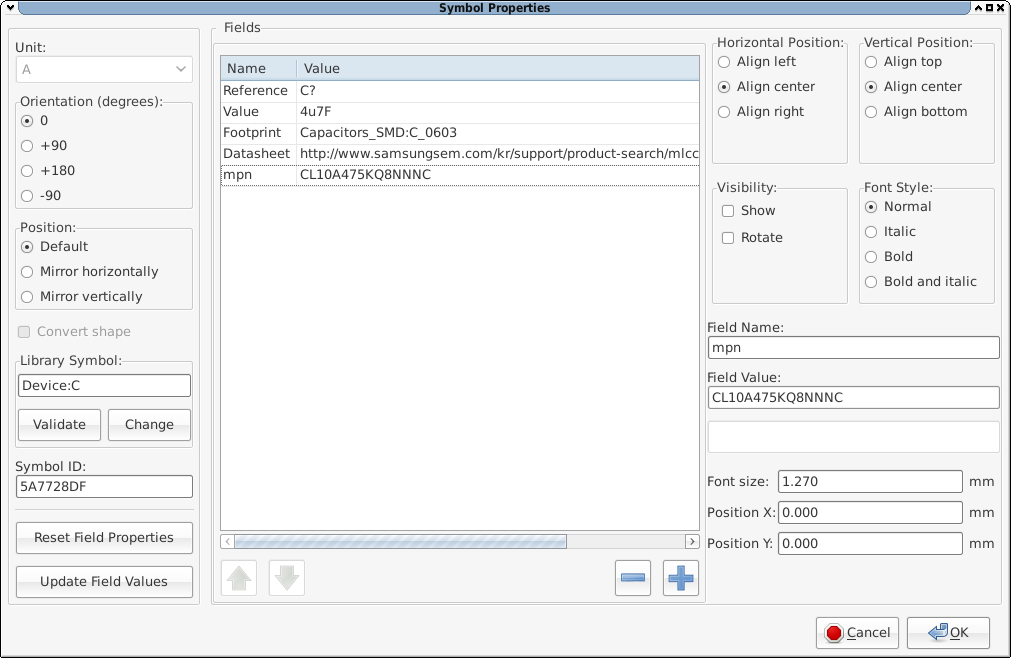
\includegraphics{chapter11/6-EditSymbolFinished.png}
	\caption[fig:symbprop]{Editing the Symbol Properties}
\end{figure}

It is a good idea to add the MPN to each part while you are building the circuit.
This ensures that your schematic matches the reality of which parts are available to you.
Often, if you design a schematic without MPN, you will find at the end that you need to substitute a number of components due to availability issues, incompatibility or other problems.
Replacing components in complex circuits can often have knock-on effects when the changes cascade from one system to the next.
When and where you choose to add 

When adding parts, I like to think in terms of groupings.
These groups of components are natural starting points for subsheets in a schematic.
Most boards will have some input and some output.
The input might be external connections or a board mounted sensor or user buttons.
The output might likely be external connections or a display or a motor.

Whatever the inputs and outputs, I find it useful to group these sections separately and add the components to them individually.
In each sheet, I will add components in a roughly circular pattern around a central component.
Often, sheets will have one or two of these `pools' of component groupings.

\section{Connections}

Once you have your components in place on your schematic, you'll need to tell Eeschema how you would like them to connect.
Connections can be made directly pin-to-pin\sidenote{Most designers will only use this sort of shortcut in the case of a power pin; either voltage supply or ground reference.} or via an intermediate wire.
Connections can also be implied by the use of labels to denote which wires are electrically connected without being graphically connected.

There is no hard and fast rule for how to lay out the connections between pins.
Just as there are no rules set in stone for how one should construct a sentence or paragraph or novel.
But just as there are novels that are enjoyable and those that are not, so too are there schematics that are informative, enlightening and helpful.
And those that are not.

General do-rules for good schematic design
\begin{enumerate}
\item Group schematic items by function.
\item Use global power labels for power connections.
\item Label any wire that goes between active components.
\item Use busses for groups of functionally related connections.
\item Use symmetry when laying out similar parts and functions.
\end{enumerate}

General do-\textbf{not}-rules for good schematic design
\begin{enumerate}
\item Do not cross wires more than absolutely necessary.
\item Do not be cramped.
\end{enumerate}

\subsection{Wires}

\subsection{Busses}
\subsection{Labels}
\subsection{Junctions}
\subsection{No Connects}
\subsection{Hierarchical Pins}

\section{Electrical Rules Check}

\section{Graphical Elements}

\section{Templates}

\section{Schematic Editor Examples}
\subsection{Example 1: Single Page Schematic}
\subsection{Example 2: Hierarchical Schematic}